% Created 2019-06-05 Wed 06:15
% Intended LaTeX compiler: pdflatex
\documentclass[dvipdfmx,10pt]{article}
\usepackage[utf8]{inputenc}
\usepackage[T1]{fontenc}
\usepackage{graphicx}
\usepackage{grffile}
\usepackage{longtable}
\usepackage{wrapfig}
\usepackage{rotating}
\usepackage[normalem]{ulem}
\usepackage{amsmath}
\usepackage{textcomp}
\usepackage{amssymb}
\usepackage{capt-of}
\usepackage{hyperref}
%% Margin
%% \usepackage[margin=1.5cm]{geometry}
\usepackage[top=1.5cm, bottom=1.5cm, left=1.5cm, right=1.5cm, headsep=4pt]{geometry}
%% \addtolength{\topmargin}{0.3cm}
%% \addtolength{\textheight}{1.75in}
%% Math
\usepackage{amsmath}
\usepackage{amssymb}
\usepackage{wasysym}
%% Allow new page within align
\allowdisplaybreaks
\usepackage{cancel}
% % Code
\usepackage{listings}
\usepackage{courier}
\lstset{basicstyle=\footnotesize\ttfamily, breaklines=true, frame=single}
\usepackage[cache=false]{minted}
\usemintedstyle{vs}
%% Graphics
\usepackage{graphicx}
\usepackage{grffile}
%% DAG
\usepackage{tikz}
\usetikzlibrary{positioning,shapes.geometric}
%% Date
\usepackage[yyyymmdd]{datetime}
\renewcommand{\dateseparator}{--}
%% Header
\usepackage{fancyhdr}
\pagestyle{fancy}
\fancyhf{} % Erase first to supress section names
\fancyhead[L]{Kazuki Yoshida} % LEFT
\fancyhead[C]{} % CENTER
\fancyhead[R]{\today} % RIGHT
\fancyfoot[C]{\thepage}
%% \fancyfoot[R]{Page \thepage\ of \pageref{LastPage}}
%% Section font size
\usepackage{sectsty}
\sectionfont{\small}
\subsectionfont{\small}
\subsubsectionfont{\small}
%% Section numbering
%% http://tex.stackexchange.com/questions/3177/how-to-change-the-numbering-of-part-chapter-section-to-alphabetical-r
%% \renewcommand\thesection{\alph{section}}
%% \renewcommand\thesubsection{\thesection.\arabic{subsection}}
%% \renewcommand{\thesubsubsection}{\thesubsection.\alph{subsubsection}}
%%
%% http://tex.stackexchange.com/questions/40067/numbering-sections-with-sequential-integers
%% \usepackage{chngcntr}
%% \counterwithout{subsection}{section}
%% enumerate
\usepackage{enumerate}
%% double space
%% \usepackage{setspace}
%% \linespread{2}
%% Paragraph Indentation
\usepackage{indentfirst}
\setlength{\parindent}{0em}
%% Spacing after headings
%% http://tex.stackexchange.com/questions/53338/reducing-spacing-after-headings
\usepackage{titlesec}
\titlespacing      \section{0pt}{12pt plus 4pt minus 2pt}{0pt plus 2pt minus 2pt}
\titlespacing   \subsection{0pt}{12pt plus 4pt minus 2pt}{0pt plus 2pt minus 2pt}
\titlespacing\subsubsection{0pt}{12pt plus 4pt minus 2pt}{0pt plus 2pt minus 2pt}
%% Fix figures and tables by [H]
\usepackage{float}
%% Allow URL embedding
\usepackage{url}
\usepackage{fontawesome}
\input{\string~/.emacs.d/misc/GrandMacros}
\author{Kazuki Yoshida \\ \\ \faTwitter \href{https://twitter.com/kaz\_yos}{@kaz\_yos} \faGithub \href{https://github.com/kaz-yos/}{kaz-yos}}
\date{\today\\}
\title{Review of Positivity with Continuous Exposure}
\hypersetup{
 pdfauthor={Kazuki Yoshida \\ \\ \faTwitter \href{https://twitter.com/kaz\_yos}{@kaz\_yos} \faGithub \href{https://github.com/kaz-yos/}{kaz-yos}},
 pdftitle={Review of Positivity with Continuous Exposure},
 pdfkeywords={},
 pdfsubject={},
 pdfcreator={Emacs 27.0.50 (Org mode 9.2.3)}, 
 pdflang={English}}
\begin{document}

\maketitle
\sloppy
\section{INTRODUCTION}
\label{sec:orgcdbb454}
\subsection{Positivity and continuous exposure}
\label{sec:org19b1033}
\begin{itemize}
\item Here we will review meaning and implication of positivity violation when the exposure of interest is continuous.
\item Special thanks to \href{https://twitter.com/EpiDancer/status/1135741241386328065}{@EpiDancer}, \href{https://twitter.com/ashley\_naimi/status/1136045624724529153}{@ashley\_naimi}, and \href{https://twitter.com/jfeldman\_epi/status/1136116613630103553}{@jfeldman\_epi}.
\end{itemize}

\subsection{Notations}
\label{sec:org5c8b59d}
\begin{align*}
  Y &: \text{Outcome measured at the end of the study}\\
  Y^{a_{0}} &: \text{Counterfactual outcome with intervention at time 0 only}\\
  Y^{a_{0},a_{1}} &: \text{Counterfactual outcome with intervention at time 0 and 1}\\
  L_{0} &: \text{Baseline covariates}\\
  A_{0} &: \text{Baseline treatment assignment}\\
  L_{1} &: \text{Post-baseline covariates}\\
  A_{1} &: \text{Post-baseline treatment assignment}\\
\end{align*}

Here we will only consider the causal effect of \(A_{0}\) and its associated counterfactual \(Y^{a_{0}}\).

\subsection{Causal structure}
\label{sec:orgcb7d0b6}
\begin{enumerate}
\item Original DAG
\label{sec:org9339ce2}
\begin{center}
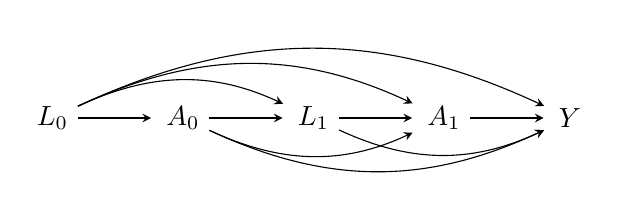
\begin{tikzpicture}[%
  ->,
  shorten >=2pt,
  >=stealth,
  node distance=1cm,
  pil/.style={
    ->,
    thick,
    shorten =2pt,}
  ]
  %% Nodes
  \node (L0) {$L_{0}$};
  \node[right = 1cm of L0] (A0) {$A_{0}$};
  \node[right = 1cm of A0] (L1) {$L_{1}$};
  \node[right = 1cm of L1] (A1) {$A_{1}$};
  \node[right = 1cm of A1] (Y) {$Y$};
  %% Edges
  \draw[->] (L0) to (A0);
  \draw[->] (L0) to [out=25,in=155] (L1);
  \draw[->] (L0) to [out=25,in=155] (A1);
  \draw[->] (L0) to [out=25,in=155] (Y);
  \draw[->] (A0) to (L1);
  \draw[->] (A0) to [out=-25,in=-155] (A1);
  \draw[->] (A0) to [out=-25,in=-155] (Y);
  \draw[->] (L1) to (A1);
  \draw[->] (L1) to [out=-25,in=-155] (Y);
  \draw[->] (A1) to (Y);
\end{tikzpicture}
\end{center}

\item Single time point intervention SWIG
\label{sec:orga099423}
\begin{center}
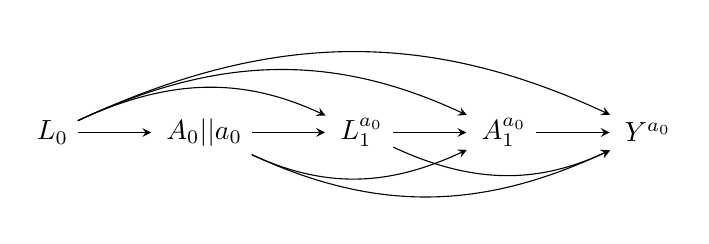
\begin{tikzpicture}[%
  ->,
  shorten >=2pt,
  >=stealth,
  node distance=1cm,
  pil/.style={
    ->,
    thick,
    shorten =2pt,}
  ]
  %% Nodes
  \node (L0) {$L_{0}$};
  \node[right = 1cm of L0] (A0) {$A_{0}||a_{0}$};
  \node[right = 1cm of A0] (L1) {$L_{1}^{a_{0}}$};
  \node[right = 1cm of L1] (A1) {$A_{1}^{a_{0}}$};
  \node[right = 1cm of A1] (Y) {$Y^{a_{0}}$};
  %% Edges
  \draw[->] (L0) to (A0);
  \draw[->] (L0) to [out=25,in=155] (L1);
  \draw[->] (L0) to [out=25,in=155] (A1);
  \draw[->] (L0) to [out=25,in=155] (Y);
  \draw[->] (A0) to (L1);
  \draw[->] (A0) to [out=-25,in=-155] (A1);
  \draw[->] (A0) to [out=-25,in=-155] (Y);
  \draw[->] (L1) to (A1);
  \draw[->] (L1) to [out=-25,in=-155] (Y);
  \draw[->] (A1) to (Y);
\end{tikzpicture}
\end{center}

The backdoor to \(A_{0}\) is only through \(L_{0}\). Thus, conditioning on \(L_{0}\) is sufficient for exchangeability as explained below.
\end{enumerate}

\section{Single time point strategy}
\label{sec:org3660bcc}
\subsection{Identifiability Conditions}
\label{sec:orgb817369}
We will follow the terminologies in \cite{hernanCausalInference2019} (Chapter 3).
\begin{itemize}
\item \textbf{Consistency}: the values of treatment under comparison correspond to well-defined interventions that, in turn, correspond to the versions of treatment in the data
\end{itemize}
\begin{center}
\(Y_{i} = Y_{i}^{a_{0}}\) if \(A_{0i} = a_{0}\) for all \(a_{0}\)
\end{center}
\begin{itemize}
\item \textbf{Exchangeability}: the conditional density of receiving every value of treatment, though not decided by the investigators, depends only on the measured covariates
\end{itemize}
\begin{center}
\(A_{0} \ind Y^{a_{0}} | L_{0}\) for all \(a_{0}\)
\end{center}
\begin{itemize}
\item \textbf{Positivity}: the conditional density of receiving every value of treatment is greater than zero, i.e., positive
\end{itemize}
\begin{center}
\(f(A_{0} = a_{0} | L_{0} = l_{0}) > 0\) for all \(a_{0},l_{0}\) where \(f(L_{0} = l_{0}) > 0\)
\end{center}

\subsection{Identification with all conditions met}
\label{sec:org9a31f35}
Here we will examine how the average causal effect is identified when all three conditions are met. Please note identification REF is under infinite amount of data. This derivation follows the Technical Point 2.3 in \cite{hernanCausalInference2019}.
\begin{align*}
  &~~~\text{By iterative expectation}\\
  E[Y^{a_{0}}]
  &= E[E[Y^{a_{0}} | L_{0}]]\\
  &~~~\text{By conditional exchangeability: } Y^{a_{0}} \ind A_{0} | L_{0}\\
  &= E[E[Y^{a_{0}} | A_{0}, L_{0}]]\\
  &~~~\text{By exchangeability, }E[Y^{a_{0}} | A_{0}, L_{0}] = E[Y^{a_{0}} | A_{0} = a_{0}, L_{0}]\\
  &= E[E[Y^{a_{0}} | A_{0} = a_{0}, L_{0}]]\\
  &~~~\text{By consistency}\\
  &= E[E[Y | A_{0} = a_{0}, L_{0}]]\\
  &~~~\text{Make outer expectation explicit integration}\\
  &= \int_{l_{0}} E[Y | A_{0} = a_{0}, L_{0} = l_{0}] f(L_{0} = l_{0}) \text{d}l_{0}\\
  &= \text{Conditional mean averaged over $L_{0}$}\\
\end{align*}
The role of positivity is to ensure that the last integration is well defined at all \(l_{0}\) values with \(f(L_{0} = l_{0}) > 0\) for any given \(a_{0}\). As a result, we can identify the mean counterfactual outcome in the population at any given \(a_{0}\) with observable variables. Thus, any causal contrast of interest \(E[Y^{a_{0}}] - E[Y^{a_{0}*}]\) is also identifiable. This also implies the entire counterfactual dose response (functional form of \(E[Y^{a_{0}}]\) as a function of \(a_{0}\)) in the population is identified.

\subsection{Non-identification with positivity violation}
\label{sec:orgf7e27df}
Here we will examine the implication of positivity violation, which is the complement of the positivity condition stated above.

\begin{itemize}
\item \textbf{Positivity violation}: the conditional density of receiving some value of treatment is not greater than zero
\end{itemize}
\begin{center}
\(f(A_{0} = a_{0} | L_{0} = l_{0}) = 0\) for some \(a_{0},l_{0}\) where \(f(L_{0} = l_{0}) > 0\)
\end{center}

The identification formula is still the same.
\begin{align*}
  &~~~\text{By iterative expectation}\\
  E[Y^{a_{0}}]
  &= E[E[Y^{a_{0}} | L_{0}]]\\
  &~~~\text{By conditional exchangeability: } Y^{a_{0}} \ind A_{0} | L_{0}\\
  &= E[E[Y^{a_{0}} | A_{0}, L_{0}]]\\
  &~~~\text{By exchangeability, }E[Y^{a_{0}} | A_{0}, L_{0}] = E[Y^{a_{0}} | A_{0} = a_{0}, L_{0}]\\
  &= E[E[Y^{a_{0}} | A_{0} = a_{0}, L_{0}]]\\
  &~~~\text{By consistency}\\
  &= E[E[Y | A_{0} = a_{0}, L_{0}]]\\
  &~~~\text{Make outer expectation explicit integration}\\
  &= \int_{l_{0}} E[Y | A_{0} = a_{0}, L_{0} = l_{0}] f(L_{0} = l_{0}) \text{d}l_{0}\\
  &= \text{Conditional mean averaged over $L_{0}$}\\
\end{align*}

The last integration is not always well defined. At some values of \(a_{0}\), \(E[Y | A_{0} = a_{0}, L_{0} = l_{0}]\) is undefined or unobservable at some \(l_{0}\) where \(f(L_{0} = l_{0}) > 0\) because \(f(A_{0} = a_{0} | L_{0} = l_{0}) = 0\). Therefore, the counterfactual dose response in the population is not identifiable. However, some specific causal contrasts may be identifiable. For two specific exposure values \(a_{0}\) and \(a_{0}*\) that both satisfy positivity at all \(l_{0}\) where \(f(L_{0} = l_{0}) > 0\), we can identify \(E[Y^{a_{0}}] - E[Y^{a_{0}*}]\).

\subsection{Illustration with a toy example}
\label{sec:orgd3db077}

Consider a continuous exposure \(A_{0}\) and a continuous \(L_{0}\) that both take on values between 0 and 1. We assume \(f(L_{0} = l_{0}) > 0\) for all values between 0 and 1. We further assume the exposure density is positive only in the shaded area in the figure.

\scriptsize
\begin{minted}[frame=lines,linenos=false]{r}
library(tidyverse)
tibble(x = seq(from = 0, to = 1, by = 0.01),
       ymin = 0   + 0.4 * x,
       ymax = 0.6 + 0.4 * x) %>%
ggplot(mapping = aes(x = x)) +
  geom_ribbon(mapping = aes(ymin = ymin, ymax = ymax),
              alpha = 0.5, fill = "gray") +
  labs(y = "A0", x = "L0") +
  scale_y_continuous(breaks = seq(from = 0, to = 1, by = 0.1)) +
  theme_bw() +
  theme(axis.text.x = element_text(angle = 0, vjust = 0.5),
        legend.key = element_blank(),
        plot.title = element_text(hjust = 0.5),
        strip.background = element_blank())
\end{minted}

\begin{center}
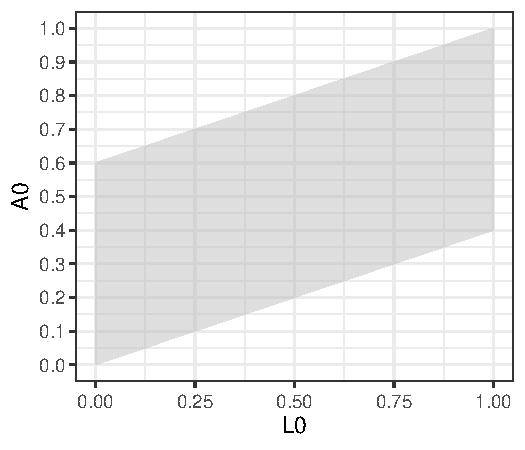
\includegraphics[page=1,keepaspectratio,width=0.5\textwidth,height=\textheight]{./source/positivity_figure1.pdf}
\end{center}
\normalsize

At \(L_{0} = 0\), \(A_{0}\) can only take on values between 0 and 0.6. At \(L_{0} = 1\), \(A_{0}\) can only take on values between 0.4 and 1.0. That is, although \(A_{0}\) does vary over the full range between 0 and 1 in the population, the range of values that \(A_{0}\) can take on is restricted at any given \(L_{0}=l_{0}\) value. We will consider what counterfactual quantities and causal effects are identifiable.\\

\begin{enumerate}
\item \(E[Y^{a_{0}}]\) for \(a_{0} < 0.4\)
\label{sec:org2cbb7ae}
\begin{align*}
  E[Y^{a_{0}}]
  &= \int_{l_{0}} E[Y | A_{0} = a_{0}, L_{0} = l_{0}] f(L_{0} = l_{0}) \text{d}l_{0}\\
\end{align*}
For exposure values below 0.4, the above identification formula is not well defined as the shaded positive area does not span the entire width of \(L_{0}\) distribution (lower triangular white area violates positivity) and some of the conditional expectations are undefined.

\item \(E[Y^{a_{0}}]\) for \(a_{0} > 0.6\)
\label{sec:org5ded2f8}
\begin{align*}
  E[Y^{a_{0}}]
  &= \int_{l_{0}} E[Y | A_{0} = a_{0}, L_{0} = l_{0}] f(L_{0} = l_{0}) \text{d}l_{0}\\
\end{align*}
For exposure values above 0.6, the above identification formula is not well defined as the shaded positive area does not span the entire width of \(L_{0}\) distribution (upper triangular white area violates positivity) and some of the conditional expectations are undefined.

\item \(E[Y^{a_{0}}]\) for \(0.4 \le a_{0} \le 0.6\)
\label{sec:org9326494}
\begin{align*}
  E[Y^{a_{0}}]
  &= \int_{l_{0}} E[Y | A_{0} = a_{0}, L_{0} = l_{0}] f(L_{0} = l_{0}) \text{d}l_{0}\\
\end{align*}
For exposure values between 0.4 and 0.6, the above identification formula is well defined as the shaded positive area does span the entire width of \(L_{0}\) distribution. All necessary conditional expectations are defined and observable. Therefore, the population counterfactual dose response in this restricted [0.4, 0.6] range is identifiable. Any causal contrast \(E[Y^{a_{0}}] - E[Y^{a_{0}*}]\) for specific values \(a_{0}\) and \(a_{0}*\) both of which are within the [0.4, 0.6] range is identified.

\item \(E[Y^{a_{0}} | L_{0} \le 0.5]\)
\label{sec:org0c596f7}
\begin{align*}
  E[Y^{a_{0}} | L_{0} \le 0.5]
  &= \int_{0}^{0.5} E[Y | A_{0} = a_{0}, L_{0} = l_{0}] f(L_{0} = l_{0}) \text{d}l_{0}\\
\end{align*}

If we limit the inference to a subset of the population where \(L_{0} \le 0.5\), the range of values for \(a_{0}\) where the mean counterfactual outcome is identified expands.

For exposure values between 0.2 and 0.6, the above identification formula is well defined as the shaded positive area does span the left half of of \(L_{0}\) distribution. All necessary conditional expectations are defined and observable. Therefore, the subpopulation counterfactual dose response in this restricted [0.2, 0.6] range is identifiable. Any causal contrast \(E[Y^{a_{0}} | L_{0} \le 0.5] - E[Y^{a_{0}*} | L_{0} \le 0.5]\) for specific values \(a_{0}\) and \(a_{0}*\) both of which are within the [0.2, 0.6] range is identified.
\end{enumerate}


\section{Bibliography Part}
\label{sec:orge3655d0}
\subsection{Bibliography}
\label{sec:orgf998314}
\renewcommand{\section}[2]{}

\bibliographystyle{apalike}
\bibliography{../../../.emacs.d/misc/zotero}
\end{document}